\documentclass{beamer}

\usepackage[french]{babel}

\usepackage[T1]{fontenc}

\usepackage[utf8]{inputenc}
\usepackage{verbatim}				%Citation de code
\usepackage{moreverb}				%Citation de code
\let\verbatiminput=\verbatimtabinput


%\pgfpagesuselayout{4 on 1}[landscape,a4paper,border shrink=5mm]

\usetheme{Warsaw}

\title [Projet noté] {Projet Noté\\
\large\emph{Algorithmes Avancés}}
\author {José Ferro Pinto\and Fabrice Ceresa}
\institute {HEPIA}
\date {\today}
\titlegraphic{
\includegraphics[height=10mm]{scikit-learn-logo-small.png}}
\logo{
\includegraphics[height=5mm]{logo-footer.png}}


\begin{document}
    \begin{frame}
        \titlepage
    \end{frame}
    
    \begin{frame}
        \frametitle{Partie 1}
        \framesubtitle{Datasets}
        Titanic :
        \begin{itemize}
         \item Nombre de données : 2201
         \item Nombre de classes: 2 (Survived or Died)
         \item Dimensionalité : 3 (billet, âge, sexe)
        \end{itemize}
    \end{frame}
    
    \begin{frame}[fragile]
        \frametitle{Partie 1}
        \framesubtitle{Méthodologie}
        \begin{itemize}
            \item \verb?KMeans?
            \item Paramètres fixes : \verb?init='random'?, \verb?random_state=0?
        
            \item Paramètre variable : \verb?n_clusters? nombre de clusters [1,25] avec un pas de 1
        \end{itemize}
    \end{frame}
    
    \begin{frame}[fragile]
        \frametitle{Partie 1}
        \framesubtitle{Résultats}
        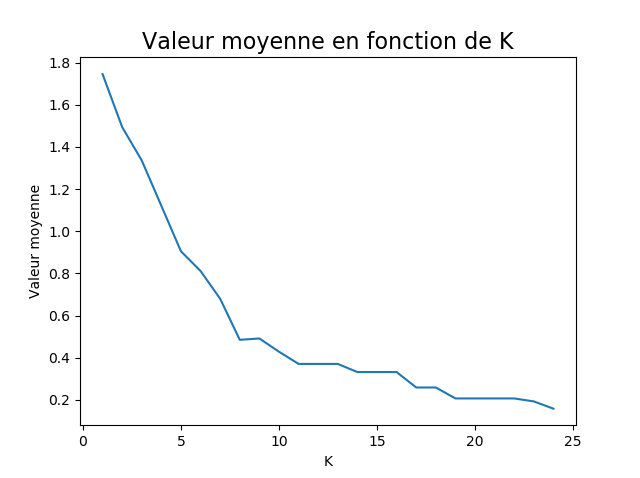
\includegraphics[scale=0.6]{p1-1}
    \end{frame}
    
    \begin{frame}[fragile]
        \frametitle{Partie 1}
        \framesubtitle{Résultats}
        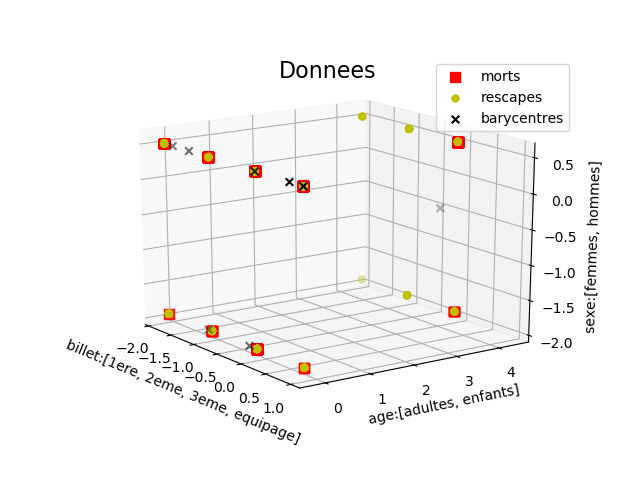
\includegraphics[scale=0.6]{p1-2}
    \end{frame}
    
    \begin{frame}[fragile]
        \frametitle{Partie 1}
        \framesubtitle{Résultats}
        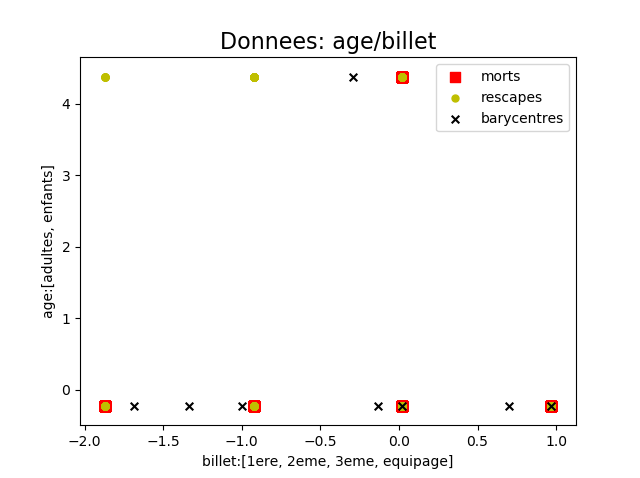
\includegraphics[scale=0.6]{p1-3}
    \end{frame}
    
    \begin{frame}[fragile]
        \frametitle{Partie 1}
        \framesubtitle{Résultats}
        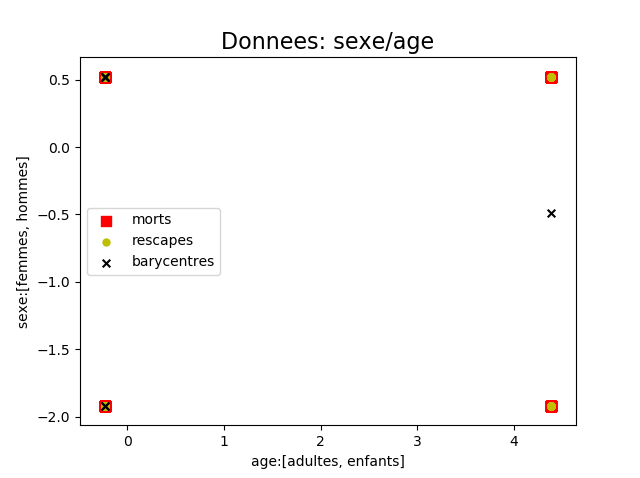
\includegraphics[scale=0.6]{p1-4}
    \end{frame}
    
    \begin{frame}[fragile]
        \frametitle{Partie 1}
        \framesubtitle{Résultats}
        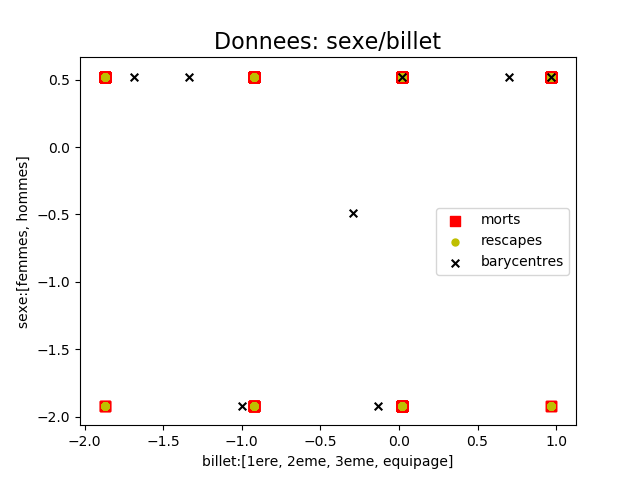
\includegraphics[scale=0.6]{p1-5}
    \end{frame}
    
    \begin{frame}
        \frametitle{Partie 2}
        \framesubtitle{Datasets}
        Cancer du sein du Wisconsin :
        \begin{itemize}
         \item Nombre de données : 569
         \item Nombre de classes: 2 (Malignant or Benign)
         \item Dimensionalité : 30
        \end{itemize}
        Vin :
        \begin{itemize}
         \item Nombre de données : 178
         \item Nombre de classes: 3
         \item Dimensionalité : 13
        \end{itemize}
    \end{frame}
    
    \begin{frame}
        \frametitle{Partie 2}
        \framesubtitle{Méthodologie}
        
        Le programme se passe en 4 boucles intriquées :
        \begin{enumerate}
            \item Pour chacun des datasets
            \item Pour chacun des classificateurs
            \item Pour chacun des paramètres
            \item Pour chacune des étapes de la validation croisée
        \end{enumerate}
    \end{frame}
    
    \begin{frame}[fragile]
        \frametitle{Partie 2}
        \framesubtitle{Classificateur : K-plus proches voisins}
        \begin{itemize}
            \item \verb?KNeighborsClassifier?
            \item Paramètre variable : \verb?n_neighbors? nombre de voisins pris en compte : [1,51] avec un pas de 5
        \end{itemize}
    \end{frame}
    
    \begin{frame}[fragile]
        \frametitle{Partie 2}
        \framesubtitle{Classificateur : arbres de décisions}
        \begin{itemize}
            \item \verb?DecisionTreeClassifier?
            \item Paramètre variable: \verb?min_samples_leaf? Nombre d'objets à partir duquel on comptabilise une feuille [2, 52] avec un pas de 5
        \end{itemize}
    \end{frame}

    \begin{frame}[fragile]
        \frametitle{Partie 2}
        \framesubtitle{Classificateur : Perceptron multi-couche avec une couche utilisant ``stochastic gradient descent''}
        \begin{itemize}
            \item \verb?MLPClassifier?
            \item Paramètres fixes : \verb?solver='sgd'?, \verb?activation='logistic'?, \verb?max_iter=1000?, \verb?verbose=False?, \verb?learning_rate_init=0.1?, \verb?tol=0.?, \verb?early_stopping=True?
        
            \item Paramètre variable : \verb?hidden_layer_sizes=(nodes,)? donc une couche et nodes varie entre 2 et 20 par pas de 3.
        \end{itemize}
    \end{frame}
    
    \begin{frame}[fragile]
        \frametitle{Partie 2}
        \framesubtitle{Classificateur : Perceptron multi-couche avec une couche utilisant ``a stochastic gradient-based optimizer''}
        \begin{itemize}
            \item \verb?MLPClassifier?
            \item Paramètres fixes : \verb?solver='adam'?, \verb?activation='logistic'?, \verb?max_iter=1000?, \verb?verbose=False?, \verb?learning_rate_init=0.1?, \verb?tol=0.?, \verb?early_stopping=True?
        
            \item Paramètre variable : \verb?hidden_layer_sizes=(nodes,)? donc une couche et nodes varie entre 2 et 20 par pas de 3.
        \end{itemize}
    \end{frame}
    
    \begin{frame}[fragile]
        \frametitle{Partie 2}
        \framesubtitle{Classificateur : Perceptron multi-couche avec deux couches utilisant ``a stochastic gradient-based optimizer''}
        \begin{itemize}
            \item \verb?MLPClassifier?
            \item Paramètres fixes : \verb?solver='adam'?, \verb?activation='logistic'?, \verb?max_iter=1000?, \verb?verbose=False?, \verb?learning_rate_init=0.1?, \verb?tol=0.?, \verb?early_stopping=True?
        
            \item Paramètre variable :  \verb?hidden_layer_sizes=(nodes, 5)? donc deux couches et nodes varie entre 2 et 20 par pas de 3.
        \end{itemize}
    \end{frame}
    
    \begin{frame}[fragile]
        \frametitle{Partie 2}
        \framesubtitle{Validation : Validation croisée}
        \begin{center}
            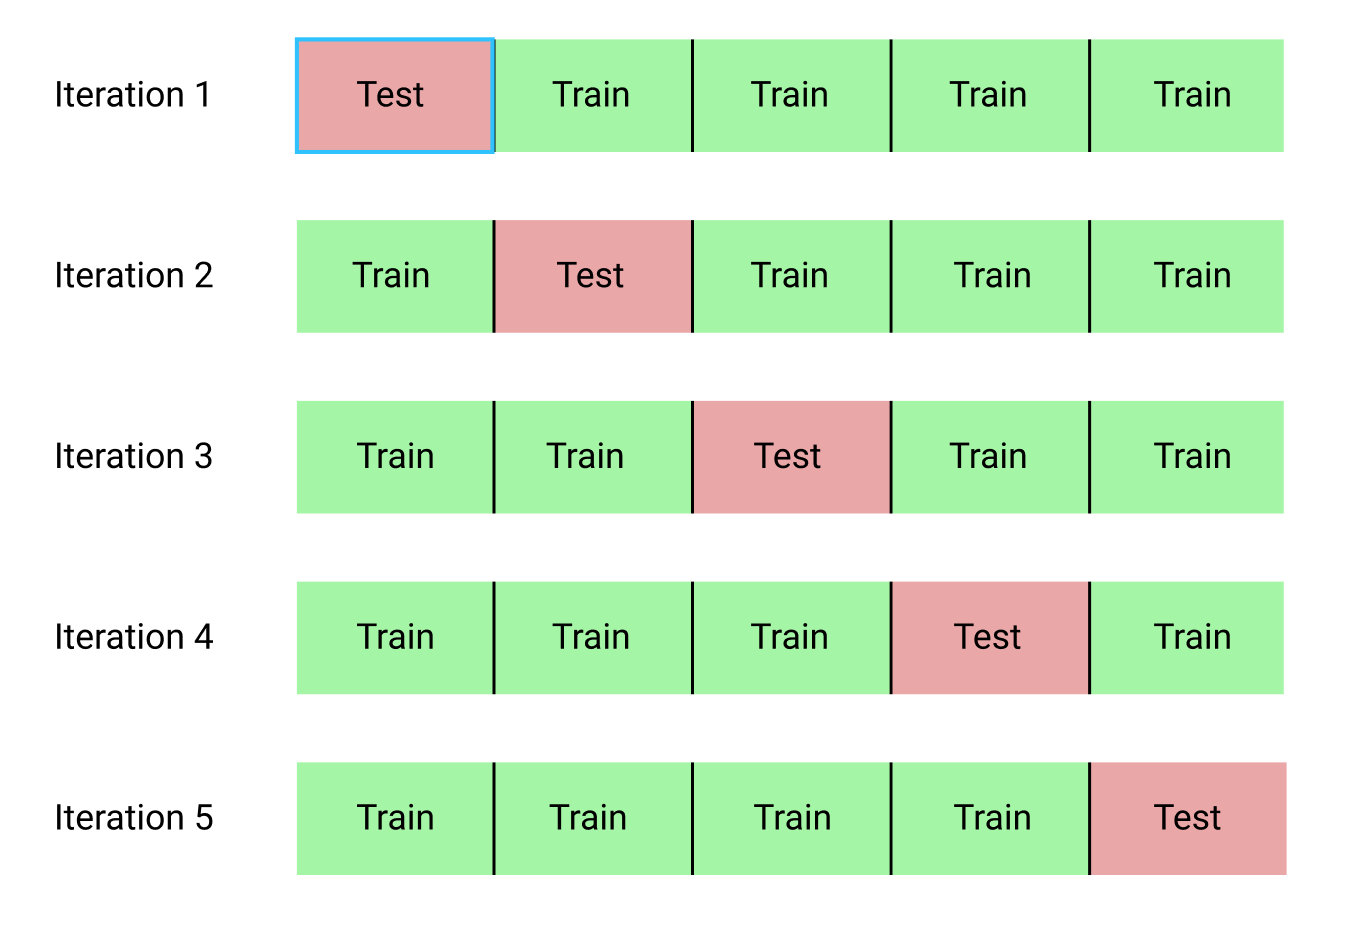
\includegraphics[scale=0.25]{kfold}
        \end{center}

        Utilisation de \verb?RepeatedKFold(n_splits=5, n_repeats=10, random_state=None)?
    \end{frame}
    
    \begin{frame}[fragile]
        \fontsize{7}{7.2}\selectfont
        \frametitle{Partie 2}
        \framesubtitle{Resultats : Cancer du sein}
        \verbatiminput{p2breast.txt}
    \end{frame}
    
    \begin{frame}[fragile]
        \fontsize{7}{7.2}\selectfont
        \frametitle{Partie 2}
        \framesubtitle{Resultats : Vin}
        \verbatiminput{p2wine.txt}
    \end{frame}
    
    \begin{frame}[fragile]
        \frametitle{Partie 2}
        \framesubtitle{Conclusions}
        \begin{itemize}
            \item Echantillonnage plus grand (569 vs 178) $\Rightarrow$ meilleurs résultats
            \begin{itemize}
                \item score moyen général : 0.830857845 vs 0.565530503
                \item écart-type moyen général : 0.011719923 vs 0.033507676
            \end{itemize}
            \item Moins échantillon $\Rightarrow$ plus rapide
            \item Plus lent $\nRightarrow$ meilleurs résultats
        \end{itemize}
    \end{frame}
    
    \begin{frame}
        \frametitle{Partie 3}
        \framesubtitle{Dataset}
        Letter Image Recognition Data\footnote{\url{https://archive.ics.uci.edu/ml/datasets/Letter+Recognition}}
        \begin{itemize}
            \item Nombre de données : 20000
            \item Nombre de classes: 26 (1 par lettre)
            \item Dimensionalité : 16
        \end{itemize}
    \end{frame}
    
    \begin{frame}
        \frametitle{Partie 3}
        \framesubtitle{Méthodologie}
        \begin{itemize}
            \item Transformation de lettres vers numéro
            \item import des données avec \verb?numpy.genfromtxt()?
            \item Reprise du travail de la partie 2
        \end{itemize}
    \end{frame}
    
    \begin{frame}[fragile]
        \fontsize{7}{7.2}\selectfont
        \frametitle{Partie 3}
        \framesubtitle{Resultats}
        \verbatiminput{partie3.txt}
    \end{frame}
    
    \begin{frame}[fragile]
        \frametitle{Partie 3}
        \framesubtitle{Conclusions}
        \begin{itemize}
            \item Résultats beaucoup plus variables
            \item Perceptron travaille longtemps pour un résultat pas très probant ($\sim$0.66)
            \item Arbre de décision ($\sim$0.73)
            \item K-plus proches voisins ($\sim$0.92)
        \end{itemize}
    \end{frame}
\end{document}
